\documentclass[10pt]{article}
\usepackage[left=1.5cm,top=1.5cm,right=1.5cm,bottom=1.5cm]{geometry}

\usepackage{mathtools}
\usepackage{amsmath}
\usepackage{amssymb}
\usepackage{relsize}
\DeclareMathSizes{10}{12}{7}{5}

\usepackage{polski}
\usepackage{indentfirst}
\usepackage{fontspec}
\usepackage{setspace}
\setmainfont{Verdana}
\thispagestyle{empty}

\begin{document}
\setlength{\parindent}{0cm}
\setstretch{1.3}

%\title{Laboratorium problemowe}
%\maketitle

\section*{Model matematyczny suwnicy}
\subsection*{Sformułowanie równań}
\begin{center}
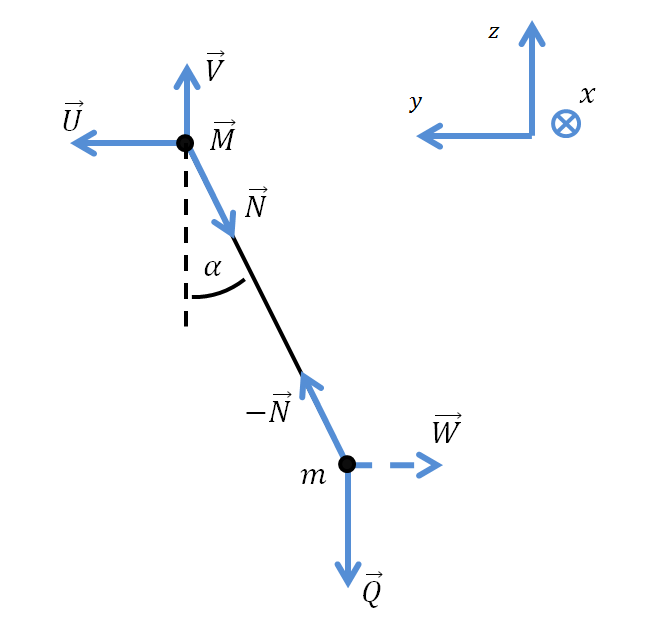
\includegraphics[width=9cm]{pic1}
\end{center}

Model opisać można za pomocą czterech równań. Pierwsze nich wynika z przedstawienia zależności między przyspieszeniem $\vec{a}_M$ cięgnika / pomostu na suwnicy symbolizowanego przez masę $\vec{M}$ (powód użycia wektora został przedstawiony dalej), a odpowiednimi siłami, które na niego działają:
\begin{equation}
\vec{U} + \vec{V} + \vec{N} + \vec{B} = \vec{M} \bullet \vec{a}_M
\end{equation}

gdzie:

\begin{description}
\item[$\vec{U} = \begin{bmatrix} u_x & u_y & 0 \end{bmatrix}^T$] - sygnał sterujący (siła)
\item[$\vec{V} = \begin{bmatrix} 0 & 0 & v_z \end{bmatrix}^T$] - pionowa składowa siły reakcji prowadnicy
\item[$\vec{N} = \begin{bmatrix} n_x & n_y & n_z \end{bmatrix}^T$] - siła naciągu liny
\item[$\vec{B} = \begin{bmatrix} b_x (\dot{x}_M) & b_y (\dot{y}_M) & 0 \end{bmatrix}^T$] - wypadkowa siła tarć i innych oporów mechanicznych
\item[$\begin{bmatrix} x_M & y_M & z_M \end{bmatrix}^T$] - położenie cięgnika
\item[$\vec{a}_M = \begin{bmatrix} \ddot{x}_M & \ddot{y}_M & 0 \end{bmatrix}^T$] - przyspieszenie cięgnika
\item[$\vec{M} = \begin{bmatrix} m_C + m_F & m_C & 0 \end{bmatrix}$] - masa cięgnika i pomostu; zastosowany został wektor w miejsce skalarnej wielkości, aby rozróżnić sytuację, gdy poruszany jest tylko cięgnik (ruch wzdłuż współrzędnej $y$), a gdy poruszany jest cięgnik wraz z pomostem (wzdłuż współrzędnej $x$); zakładamy brak ruchu wzdłuż współrzednej $z$, więc ta składowa wektora jest równa $0$
\item[$m_C$] - masa cięgnika
\item[$m_F$] - masa pomostu
\end{description}

Drugie równanie wynika z zależności między przyspieszeniem $\vec{a}_m$ zawiesia (symbolizowanego przez masę $m$), a odpowiednimi siłami, które na to obciążenie oddziałują. Wspomniane przyspieszenie jest wyznaczane względem cięgnika, więc analizowany układ odniesienia jest układem inercjalnym, który poddany jest przyspieszeniu $\vec{a}_M$:
\begin{equation}
\vec{Q} + \vec{W} - \vec{N} = m\vec{a}_m
\end{equation}

gdzie:
\begin{description}
\item[$\vec{Q} = \begin{bmatrix} 0 & 0 & -mg \end{bmatrix}^T$] - siła grawitacji działająca na obciążenie
\item[$\vec{W} = -m\vec{a}_M$] - siła bezwładności wynikająca z inercjalności układu odniesienia
\item[$m$] - masa obciążenia
\item[$\vec{a}_m = \begin{bmatrix} \ddot{x}_m & \ddot{y}_m & \ddot{z}_m \end{bmatrix}^T$] - przyspieszenie obciążenia w inercjalnym układzie odniesienia
\end{description}

Z braku ruchu wzdłuż prostej prowadzącej przez położenia wózka i obciążenia w analizowanym inercjalnym układzie odniesienia, a także biorąc pod uwagę fakt, że siła $\vec{N}$ musi być równoległa do tej prostej, wynika trzecie równanie:
\begin{equation}
\vec{N} = \begin{bmatrix} sin(\alpha_x) \\ sin(\alpha_y) \\ -cos(\alpha) \end{bmatrix}
\big( |\vec{Q}|cos(\alpha) + |\vec{W}|sin(\alpha) \big)
\end{equation}

Rozmieszczenie kątów $\beta_x$, $\beta_y$, $\alpha_x$, $\alpha_y$ i $\alpha$ zostało przestawione na rysunku poniżej:
\begin{center}
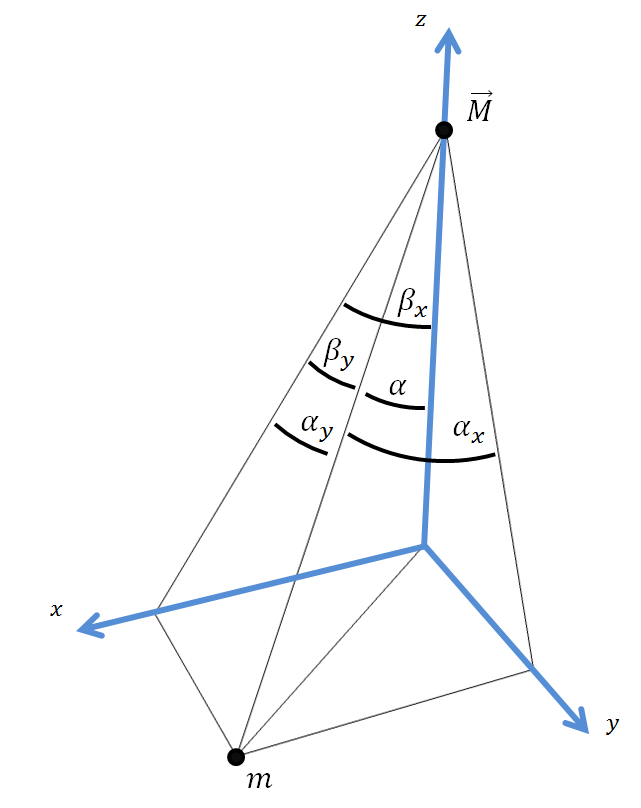
\includegraphics[width=7.5cm]{pic2mod}
\end{center}

Kąty $\alpha_x$ i $\alpha_y$ są stosowane jako zmienne stanu z uwagi na uproszczenie i symetrię modelu. W fizycznym modelu możliwy jest natomiast pomiar kątów oznaczonych jako $\beta_x$ i $\beta_y$. Oznacza to, że konieczne będzie wyznaczenie zależności umożliwiających zamianę kątów:
\begin{equation}
\begin{cases}
sin(\alpha_x) = cos(\alpha_y)sin(\beta_x) \\
a_y = b_y
\end{cases}
\end{equation}

Wyprowadzona również została zależność pozwalająca wyznaczyć kąt $\alpha$:
\begin{equation}
sin^2(\alpha_x) + sin^2(\alpha_y) = sin^2(\alpha)
\end{equation}

Po podstawieniu równania (3) oraz wszystkich pozostałych wartości do równań (1) i (2) uzyskany zostaje następujący układ równań:
\begin{equation}
\begin{bmatrix} u_x \\ u_y \\ 0 \end{bmatrix} + 
\begin{bmatrix} 0 \\ 0 \\ v_z \end{bmatrix} +
\begin{bmatrix} sin(\alpha_x) \\ sin(\alpha_y) \\ -cos(\alpha) \end{bmatrix}
\Bigg( |m\vec{g}|cos(\alpha) + m \Bigg| \begin{bmatrix} \ddot{x}_M \\ \ddot{y}_M \\ 0 \end{bmatrix}\Bigg| sin(\alpha) \Bigg) + 
\begin{bmatrix} b_x(\dot{x}_M) \\ b_y(\dot{y}_M) \\ 0 \end{bmatrix} = 
\begin{bmatrix} (m_C + m_F) \ddot{x}_M \\ m_C \ddot{y}_M \\ 0 \end{bmatrix}
\end{equation}
\begin{equation}
\begin{bmatrix} 0 \\ 0 \\ -mg \end{bmatrix} -
m \begin{bmatrix} \ddot{x}_M \\ \ddot{y}_M \\ 0 \end{bmatrix} - 
\begin{bmatrix} sin(\alpha_x) \\ sin(\alpha_y) \\ -cos(\alpha) \end{bmatrix}
\Bigg( |m\vec{g}|cos(\alpha) + m \Bigg| \begin{bmatrix} \ddot{x}_M \\ \ddot{y}_M \\ 0 \end{bmatrix} \Bigg| sin(\alpha) \Bigg)
 = m\vec{a}_m
\end{equation}

Z równań usunąć można równania dla składowej $z$, gdyż nie są one potrzebne dla dalszej analizy. Po dodatkowych uproszczeniach:

\begin{equation}
\begin{bmatrix} u_x \\ u_y \end{bmatrix} + 
m \begin{bmatrix} sin(\alpha_x) \\ sin(\alpha_y) \end{bmatrix}
\Bigg( g \cdot cos(\alpha) + \Bigg| \begin{bmatrix} \ddot{x}_M \\ \ddot{y}_M \end{bmatrix} \Bigg| sin(\alpha) \Bigg) + 
\begin{bmatrix} b_x(\dot{x}_M) \\ b_y(\dot{y}_M) \end{bmatrix} = 
\begin{bmatrix}(m_C + m_F) \ddot{x}_M \\ m_C \ddot{y}_M \end{bmatrix}
\end{equation}
\begin{equation}
 - \begin{bmatrix} \ddot{x}_M \\ \ddot{y}_M \end{bmatrix} - 
\begin{bmatrix} sin(\alpha_x) \\ sin(\alpha_y) \end{bmatrix}
\Bigg( g \cdot cos(\alpha) + \Bigg| \begin{bmatrix} \ddot{x}_M \\ \ddot{y}_M \end{bmatrix} \Bigg| sin(\alpha) \Bigg)
 = \vec{a}_m
\end{equation}

Biorąc pod uwagę, że w rzeczywistym modelu nie ma możliwości pomiaru liniowych przesunięć, prędkości ani przyspieszeń obciążenia, konieczne jest wyrażenie przyspieszenia $\vec{a}_m$ przy pomocy kątów $\alpha_x$ i $\alpha_y$ oraz długości liny $l$. Położenie względne obciążenia wyrazić można wzorem:
\begin{equation}
\vec{x}_m = l \begin{bmatrix} sin(\alpha_x) \\ sin(\alpha_y) \end{bmatrix}
\end{equation}

Przyspieszenie będzie zatem wyrażone wzorem:
\begin{equation}
\vec{a_m} = l
\begin{bmatrix}
\ddot{\alpha}_x cos(\alpha_x) - (\dot{\alpha}_x)^2 sin(\alpha_x) \\
\ddot{\alpha}_y cos(\alpha_y) - (\dot{\alpha}_y)^2 sin(\alpha_y)
\end{bmatrix}
\end{equation}

Po podstawieniu zależności (11) do równania (9) i przyrównaniu poszczególnych składowych równań (8) i (9) otrzymany zostaje następujący układ równań:

\begin{equation}
u_x + mg \cdot sin(\alpha_x) cos(\alpha) + m \cdot sin(\alpha_x) sin(\alpha) \sqrt{(\ddot{x}_M)^2 + (\ddot{y}_M)^2)} + b_x(\dot{x}_M) = (m_C + m_F) \ddot{x}_M
\end{equation}
\begin{equation}
u_y + mg \cdot sin(\alpha_y) cos(\alpha) + m \cdot sin(\alpha_y) sin(\alpha) \sqrt{(\ddot{x}_M)^2 + (\ddot{y}_M)^2)} + b_y(\dot{y}_M) = m_C \ddot{y}_M
\end{equation}
\begin{equation}
-\ddot{x_M}-sin(\alpha_x) \Big( g \cdot cos(\alpha) + sin(\alpha)\sqrt{(\ddot{x}_M)^2 + (\ddot{y}_M)^2)} \Big) = l \big( \ddot{\alpha}_x cos(\alpha_x) - (\dot{\alpha}_x)^2 sin(\alpha_x) \big)
\end{equation}
\begin{equation}
-\ddot{y}_M-sin(\alpha_y) \Big( g \cdot cos(\alpha) + sin(\alpha)\sqrt{(\ddot{x}_M)^2 + (\ddot{y}_M)^2)} \Big) = l \big( \ddot{\alpha_y} cos(\alpha_y) - (\dot{\alpha}_y)^2 sin(\alpha_y) \big)
\end{equation}

\newpage
\subsection*{Zastosowanie obliczeń numerycznych do wyznaczenia rozwiązań}
Aby możliwe było zastosowanie obliczeń numerycznych do powyższego modelu, konieczne jest przekształcenie powyższych równań, do takich postaci, aby drugie pochodne zmiennych stanu ($\ddot{x_M}, \ddot{y_M}, \ddot{\alpha_x}, \ddot{\alpha_y}$) były wyrażone w zależności od pozostałych zmiennych. W przypadku przyspieszeń kątowych, przekształcenie to jest proste, gdyż sprowadza się do drobnych przekształceń równań (14) i (15):
\begin{equation}
\ddot{\alpha_x} = \frac{1}{l \cdot cos(\alpha_x)} \bigg(l (\dot{\alpha}_x)^2 sin(\alpha_x) - \ddot{x}_M-sin(\alpha_x) \Big( g \cdot cos(\alpha) + sin(\alpha)\sqrt{(\ddot{x}_M)^2 + (\ddot{y}_M)^2)} \Big) \bigg)
\end{equation}
\begin{equation}
\ddot{\alpha_y} = \frac{1}{l \cdot cos(\alpha_y)} \bigg(l (\dot{\alpha}_y)^2 sin(\alpha_y) - \ddot{y}_M-sin(\alpha_y) \Big( g \cdot cos(\alpha) + sin(\alpha)\sqrt{(\ddot{x}_M)^2 + (\ddot{y}_M)^2)} \Big) \bigg)
\end{equation}

W przypadku przyspieszeń liniowych sprawa jest jednak bardziej skompilowana, gdyż konieczne jest rozwiązanie układu równań o postaci (ze względu na niewiadome $X$ i $Y$):
\begin{equation}
\begin{cases}
A_1+B_1\sqrt{X^2 + Y^2} = C_1X \\ 
A_2+B_2\sqrt{X^2 + Y^2} = C_2Y
\end{cases}, \quad C_1 > 0, \quad C_2 > 0
\label{eq:Primary}
\end{equation}

gdzie:
\begin{equation*}
\begin{split}
X &= \ddot{x}_M \\
Y &= \ddot{y}_M \\
A_1 &= u_x + mg \cdot sin(\alpha_x)cos(\alpha) + b_x(\dot{x}_M) \\
A_2 &= u_y + mg \cdot sin(\alpha_y)cos(\alpha) + b_y(\dot{y}_M) \\
B_1 &= m \cdot sin(\alpha_x) sin(\alpha) \\
B_2 &= m \cdot sin(\alpha_y) sin(\alpha) \\
C_1 &= m_C + m_F \\
C_2 &= m_C \\
\end{split}
\end{equation*}

\newpage
\subsubsection*{Rozwiązanie układu równań \eqref{eq:Primary}}
Rozwiązania układu równań wyrazić można w postaci:
\begin{equation}
X = R \cdot cos(\gamma), \quad Y = R \cdot sin(\gamma), \quad R \geqslant 0
\label{eq:VarChng}
\end{equation}

Po podstawieniu:
\begin{equation}
A_1 + B_1 R = C_1 R \cdot cos(\gamma), \quad
A_2 + B_2 R = C_2 R \cdot sin(\gamma)
\end{equation}

Po przekształceniu:
\begin{equation}
\frac{1}{C_1} \Big( \frac{A_1}{R} + B_1 \Big) = cos(\gamma), \quad
\frac{1}{C_2} \Big( \frac{A_2}{R} + B_2 \Big) = sin(\gamma)
\label{eg:TrigForm}
\end{equation}

Po obustronnym podniesieniu do kwadratu obu równań i zastosowaniu zależności jedynki trygonometrycznej:
\begin{equation}
\frac{1}{C_1^2} \Big( \frac{A_1}{R} + B_1 \Big)^2 + 
\frac{1}{C_2^2} \Big( \frac{A_2}{R} + B_2 \Big)^2 = 1
\end{equation}

Po uporządkowaniu zmiennych uzyskane zostaje równanie kwadratowe:
\begin{equation}
\Bigg( \frac{B_1^2}{C_1^2} + \frac{B_2^2}{C_2^2} - 1 \Bigg) R^2 +
2 \Bigg( \frac{A_1B_1}{C_1^2} + \frac{A_2B_2}{C_2^2} \Bigg) R +
\Bigg( \frac{A_1^2}{C_1^2} + \frac{A_2^2}{C_2^2} \Bigg) = 0
\end{equation}

\begin{equation}
\Delta = 4 \Bigg( \frac{A_1B_1}{C_1^2} + \frac{A_2B_2}{C_2^2} \Bigg)^2 -
4 \Bigg( \frac{B_1^2}{C_1^2} + \frac{B_2^2}{C_2^2} - 1 \Bigg)
\Bigg( \frac{A_1^2}{C_1^2} + \frac{A_2^2}{C_2^2} \Bigg)
\end{equation}

\begin{equation}
\Delta = 4 \Bigg(2
\frac{A_1 B_1 A_2 B_2}{C_1^2 C_2^2} +
\frac{A_1^2}{C_1^2} +
\frac{A_2^2}{C_2^2} -
\frac{A_1^2 B_2^2 + A_2^2 B_1^2}{C_1^2 C_2^2} 
\Bigg)
\end{equation}

\begin{equation}
\Delta = \frac{4}{C_1^2C_2^2}
\Big( 2A_1B_1A_2B_2 + A_1^2C_2^2 + A_2^2C_1^2 - A_1^2B_2^2 - A_2^2B_1^2 \Big)
\end{equation}

\begin{equation}
\Delta = \frac{4}{C_1^2C_2^2}
\Big( A_1^2C_2^2 + A_2^2C_1^2 - ( A_1B_2 - A_2B_1)^2 \Big)
\end{equation}

\begin{equation}
R_0 = \frac{-A_1B_1C_2^2 -A_2B_2C_1^2 \pm
\sqrt{A_1^2C_2^2 + A_2^2C_1^2 - ( A_1B_2 - A_2B_1)^2}}
{B_1^2C_2^2 + B_2^2C_1^2 - C_1^2C_2^2}
\end{equation}

Po podstawieniu zależności \eqref{eg:TrigForm} do \eqref{eq:VarChng} rozwiązania równania można wyrazić w postaci:
\begin{equation}
X = \frac{A_1 + B_1 R_0}{C_1}, \quad
Y = \frac{A_2 + B_2 R_0}{C_2}
\end{equation}
 
\newpage
\subsubsection*{Równania stanu}
Ostatnim krokiem przekształcenia równań do postaci możliwej do rozwiązania metodami numerycznymi jest przekształcenie ich w równania stanu, o postaci:
\begin{equation}
\dot{\vec{x}} = F(\vec{x}, \vec{u})
\end{equation}

Wektor sterowań, wektor stanu i pochodną wektora stanu wyrazić można jako:
\begin{equation}
\vec{u} = \begin{bmatrix} u_1 \\ u_2 \end{bmatrix} = \begin{bmatrix} u_x \\ u_y \end{bmatrix}, \quad
\vec{x} = 
\begin{bmatrix}
x_1 \\ x_2 \\ x_3 \\ x_4 \\ x_5 \\ x_6 \\ x_7 \\ x_8 \\
\end{bmatrix} =
\begin{bmatrix}
x_M \\ y_M \\ \alpha_x \\ \alpha_y \\ \dot{x}_M \\ \dot{y}_M \\ \dot{\alpha}_x \\ \dot{\alpha}_y
\end{bmatrix}, \quad
\dot{\vec{x}} =
\begin{bmatrix}
\dot{x}_1 \\ \dot{x}_2 \\ \dot{x}_3 \\ \dot{x}_4 \\ \dot{x}_5 \\ \dot{x}_6 \\ \dot{x}_7 \\ \dot{x}_8 \\
\end{bmatrix} =
\begin{bmatrix}
\dot{x}_M \\ \dot{y}_M \\ \dot{\alpha}_x \\ \dot{\alpha}_y \\
\ddot{x}_M \\ \ddot{y}_M \\ \ddot{\alpha}_x \\ \ddot{\alpha}_y
\end{bmatrix}
\end{equation}

Równania stanu przyjmują wtedy następującą postać:
\begin{equation}
\dot{x}_1 = x_5, \quad
\dot{x}_2 = x_6, \quad
\dot{x}_3 = x_7, \quad
\dot{x}_4 = x_8, \quad
\dot{x}_5 = X, \quad
\dot{x}_6 = Y \\
\end{equation}
\begin{equation}
\begin{split}
\dot{x}_7 &= x_7^2 tg(x_3) - \frac{X}{l \cdot cos(x_3)} - \frac{tg(x_3)}{l} \Big( g \cdot T + S\sqrt{X^2 + Y^2} \Big) \\
\dot{x}_8 &= x_8^2 tg(x_4) - \frac{Y}{l \cdot cos(x_4)} - \frac{tg(x_4)}{l} \Big( g \cdot T + S\sqrt{X^2 + Y^2} \Big)
\end{split}
\end{equation}

Gdzie:
\begin{equation}
\begin{split}
X &= \frac{A_1 + B_1 R_0}{C_1} \\
Y &= \frac{A_2 + B_2 R_0}{C_2} \\
R_0 &= \frac{-A_1B_1C_2^2 -A_2B_2C_1^2 - 
\sqrt{A_1^2C_2^2 + A_2^2C_1^2 - ( A_1B_2 - A_2B_1)^2}}
{B_1^2C_2^2 + B_2^2C_1^2 - C_1^2C_2^2} \\
A_1 &= u_1 + mg \cdot sin(x_3)T + b_x(x_5) \\
A_2 &= u_2 + mg \cdot sin(x_4)T + b_y(x_6) \\
B_1 &= m \cdot sin(x_3) S \\
B_2 &= m \cdot sin(x_4) S \\
C_1 &= m_C + m_F \\
C_2 &= m_C \\
S &= \sqrt{ sin^2(x_3) + sin^2(x_4) } \\
T &= \sqrt{1 - sin^2(x_3) - sin^2(x_4) } \\
\end{split}
\end{equation}

\newpage
\subsection*{Równania sprzężone}
\iffalse
\begin{equation}
H = \psi^T F(\vec{x},\vec{u}) = \sum_i \psi_i \dot{x}_i
\end{equation}
\begin{equation}
\dot{\psi} = - \frac{\partial H}{\partial \vec{x}}
\end{equation}
\begin{equation}
\begin{split}
\dot{\psi}_1 &= \sum_i \psi_i \frac{ \partial \dot{x}_i }{ \partial x_1 } \\
&... \\
\dot{\psi}_j &= \sum_i \psi_i \frac{ \partial \dot{x}_i }{ \partial x_j }
\end{split}
\end{equation}
\fi

W celu wyznaczenia równań sprzężonych konieczne jest obliczenie wszystkich 64 pochodnych pochodnych stanów względem stanów. Szybka analiza ujawnia jednak, że większość z tych funkcji będzie zerami, a tylko niektóre będą mieć skompilowaną postać:

\begin{center}
\begin{tabular}{c|c|c|c|c|c|c|c|c}
$\partial \dot{x}_i / \partial x_j$ &
$\dot{x}_1$ & $\dot{x}_2$ & $\dot{x}_3$ & $\dot{x}_4$ &
$\dot{x}_5$ & $\dot{x}_6$ & $\dot{x}_7$ & $\dot{x}_8$ \\ \hline
$x_1$ & $0$ & $0$ & $0$ & $0$ & $0$ & $0$ & $0$ & $0$ \\ \hline
$x_2$ & $0$ & $0$ & $0$ & $0$ & $0$ & $0$ & $0$ & $0$ \\ \hline
$x_3$ & $0$ & $0$ & $0$ & $0$ & \# & \# & \# & \# \\ \hline
$x_4$ & $0$ & $0$ & $0$ & $0$ & \# & \# & \# & \# \\ \hline
$x_5$ & $1$ & $0$ & $0$ & $0$ & \# & \# & \# & \# \\ \hline
$x_6$ & $0$ & $1$ & $0$ & $0$ & \# & \# & \# & \# \\ \hline
$x_7$ & $0$ & $0$ & $1$ & $0$ & $0$ & $0$ & \# & $0$ \\ \hline
$x_8$ & $0$ & $0$ & $0$ & $1$ & $0$ & $0$ & $0$ & \# \\
\end{tabular}
\end{center}

Pochodne w tabeli oznaczone znacznikami \# mają skomplikowane postacie i zostały obliczone poniżej:
\begin{equation}
\begin{split}
\frac{ \partial \dot{x}_5 }{ \partial x_j } &= \frac{ \partial X }{ \partial x_j }, \quad j \in \{ 3, 4, 5, 6 \} \\
\frac{ \partial \dot{x}_6 }{ \partial x_j } &= \frac{ \partial Y }{ \partial x_j }, \quad j \in \{ 3, 4, 5, 6 \} \\
\frac{ \partial \dot{x}_7 }{ \partial x_j } &= 
\frac{-1}{l \cdot cos(x_3)} \frac{\partial X}{\partial x_j} - \frac{tg(x_3)}{l} \bigg(
g \cdot \frac{\partial T}{\partial x_j} +
\frac{\partial S}{\partial x_j}\sqrt{X^2 + Y^2} +
\Big( \frac{\partial X}{\partial x_j}X + \frac{\partial Y}{\partial x_j}Y \Big) \frac{S}{\sqrt{X^2 + Y^2}} \bigg), \quad j \in \{ 4, 5, 6 \} \\
\frac{ \partial \dot{x}_8 }{ \partial x_j } &=
\frac{-1}{l \cdot cos(x_4)} \frac{\partial Y}{\partial x_j} - \frac{tg(x_4)}{l} \bigg(
g \cdot \frac{\partial T}{\partial x_j} +
\frac{\partial S}{\partial x_j}\sqrt{X^2 + Y^2} +
\Big( \frac{\partial X}{\partial x_j}X + \frac{\partial Y}{\partial x_j}Y \Big) \frac{S}{\sqrt{X^2 + Y^2}} \bigg), \quad j \in \{ 3, 5, 6 \} \\
\frac{ \partial \dot{x}_7 }{ \partial x_3 } &= \frac{l \cdot x_7^2 - \frac{\partial X}{\partial x_3} cos(x_3) -
X \cdot sin(x_3) - g \cdot T - S \sqrt{X^2 + Y^2}}{l \cdot cos^2 (x_3)} \\
&- \frac{tg(x_3)}{l} \bigg(g \cdot \frac{\partial T}{\partial x_3} + \frac{\partial S}{\partial x_3}\sqrt{X^2 + Y^2} +
\Big( \frac{\partial X}{\partial x_3}X + \frac{\partial Y}{\partial x_3}Y \Big) \frac{S}{\sqrt{X^2 + Y^2}} \bigg)  \\
\frac{ \partial \dot{x}_8 }{ \partial x_4 } &= \frac{l \cdot x_8^2 - \frac{\partial Y}{\partial x_4} cos(x_4) -
X \cdot sin(x_4) - g \cdot T - S \sqrt{X^2 + Y^2}}{l \cdot cos^2 (x_4)} \\
&- \frac{tg(x_4)}{l} \bigg(g \cdot \frac{\partial T}{\partial x_4} + \frac{\partial S}{\partial x_4}\sqrt{X^2 + Y^2} +
\Big( \frac{\partial X}{\partial x_4}X + \frac{\partial Y}{\partial x_4}Y \Big) \frac{S}{\sqrt{X^2 + Y^2}} \bigg) \\
\frac{ \partial \dot{x}_7 }{ \partial x_7 } &= 2x_7 tg(x_3) \\
\frac{ \partial \dot{x}_8 }{ \partial x_8 } &= 2x_8 tg(x_4) \\
\end{split}
\end{equation}


\newpage

% X,Y derivatives
\begin{equation}
\boldsymbol{\frac{\partial X}{\partial x_j}} = \frac{1}{C_1} \bigg(
{\frac{\partial A_1}{\partial x_j} + \frac{\partial B_1}{\partial x_j} R_0 + B_1 \frac{\partial R_0}{\partial x_j}}
\bigg), \quad
\boldsymbol{\frac{\partial Y}{\partial x_j}} = \frac{1}{C_2} \bigg(
{\frac{\partial A_2}{\partial x_j} + \frac{\partial B_2}{\partial x_j} R_0 + B_2 \frac{\partial R_0}{\partial x_j}}
\bigg)
\end{equation}

% A1 derivatives
\begin{equation}
\boldsymbol{\frac{\partial A_1}{\partial x_3}} = mg \cdot \big( cos(x_3)T + sin(x_3) \frac{\partial T}{\partial x_3} \big), \quad
\boldsymbol{\frac{\partial A_1}{\partial x_4}} = mg \cdot sin(x_3) \frac{\partial T}{\partial x_4}
\end{equation}

% A2 derivatives
\begin{equation}
\boldsymbol{\frac{\partial A_2}{\partial x_3}} = mg \cdot sin(x_4) \frac{\partial T}{\partial x_3}, \quad
\boldsymbol{\frac{\partial A_2}{\partial x_4}} = mg \cdot \big( cos(x_4)T + sin(x_4) \frac{\partial T}{\partial x_4} \big)
\end{equation}

% A1, A2 by x5, x6 derivatives
\begin{equation}
\boldsymbol{\frac{\partial A_1}{\partial x_5}} = \frac{\partial b_x}{\partial x_5}, \quad
\boldsymbol{\frac{\partial A_1}{\partial x_6}} = 0, \quad
\boldsymbol{\frac{\partial A_2}{\partial x_5}} = 0, \quad
\boldsymbol{\frac{\partial A_2}{\partial x_6}} = \frac{\partial b_y}{\partial x_6}
\end{equation}

% nonzero B1 derivatives
\begin{equation}
\boldsymbol{\frac{\partial B_1}{\partial x_3}} = m \Big(cos(x_3)S + sin(x_3) \frac{\partial S}{\partial x_3} \Big), \quad
\boldsymbol{\frac{\partial B_1}{\partial x_4}} = m \cdot sin(x_3) \frac{\partial S}{\partial x_4}
\end{equation}

% nonzero B2 derivatives
\begin{equation}
\boldsymbol{\frac{\partial B_2}{\partial x_3}} = m \cdot sin(x_4) \frac{\partial S}{\partial x_3}, \quad
\boldsymbol{\frac{\partial B_2}{\partial x_4}} = m \Big(cos(x_4)S + sin(x_4) \frac{\partial S}{\partial x_4} \Big)
\end{equation}

% zero B1, B2 derivatives
\begin{equation}
\boldsymbol{\frac{\partial B_1}{\partial x_5}} = 0, \quad
\boldsymbol{\frac{\partial B_1}{\partial x_6}} = 0, \quad
\boldsymbol{\frac{\partial B_2}{\partial x_5}} = 0, \quad
\boldsymbol{\frac{\partial B_2}{\partial x_6}} = 0
\end{equation}

% S derivatives
\begin{equation}
\boldsymbol{\frac{\partial S}{\partial x_3}} = \frac{sin(x_3) cos(x_3)}{\sqrt{ sin^2(x_3) + sin^2(x_4)} }, \quad
\boldsymbol{\frac{\partial S}{\partial x_4}} = \frac{sin(x_4) cos(x_4)}{\sqrt{ sin^2(x_3) + sin^2(x_4)} }
\end{equation}

% T derivatives
\begin{equation}
\boldsymbol{\frac{\partial T}{\partial x_3}} = \frac{-sin(x_3) cos(x_3)}{\sqrt{1 - sin^2(x_3) - sin^2(x_4)} }, \quad
\boldsymbol{\frac{\partial T}{\partial x_4}} = \frac{-sin(x_4) cos(x_4)}{\sqrt{1 - sin^2(x_3) - sin^2(x_4)} }
\end{equation}

\newpage
\subsubsection*{Wyznaczenie pochodnej $\partial R_0 / \partial x$}

Celem jest obliczenie pochodnej po $x$ wyrażenia:
\begin{equation}
R_0 = \frac{-A_1B_1C_2^2 -A_2B_2C_1^2 - 
\sqrt{A_1^2C_2^2 + A_2^2C_1^2 - ( A_1B_2 - A_2B_1)^2}}
{B_1^2C_2^2 + B_2^2C_1^2 - C_1^2C_2^2}
\end{equation}

Gdzie:
\begin{equation}
A_1 = A_1(x), \quad
A_2 = A_2(x), \quad
B_1 = B_1(x), \quad
B_2 = B_2(x), \quad
C_1 = const, \quad
C_2 = const
\end{equation}

Poprzez zastąpienie poszczególnych części tego skompilowanego wyrażenia funkcjami pomocniczymi, możliwe jest rozbicie problemu na kilka prostszych podproblemów:
\begin{equation}
R_0 = \frac{N_1-\sqrt{N_2}}{D}
\end{equation}

Gdzie:
\begin{equation}
\begin{split}
N_1 &= -A_1 B_1 C_2^2 - A_2 B_2 C_1^2 \\
N_2 &= A_1^2C_2^2 + A_2^2C_1^2 - ( A_1B_2 - A_2B_1)^2 \\
D &= B_1^2 C_2^2 + B_2^2 C_1^2 - C_1^2 C_2^2
\end{split}
\end{equation}

Wtedy:
\begin{equation}
\frac{\partial R_0}{\partial x} = \frac{1}{D^2}
\Bigg(
\bigg(
\frac{\partial N_1}{\partial x} -
\frac{1}{2} \frac{\partial N_2}{\partial x}
\frac{1}{\sqrt{N_2}}
\bigg) - 
\Big( N_1-\sqrt{N_2} \Big) \frac{\partial D}{\partial x}
\Bigg)
\end{equation}

Gdzie:
\begin{equation}
\begin{split}
\frac{\partial N_1}{\partial x} &=
-C_2^2 \bigg(\frac{\partial A_1}{\partial x} B_1 + A_1 \frac{\partial B_1}{\partial x} \bigg)
-C_1^2 \bigg(\frac{\partial A_2}{\partial x} B_2 + A_2 \frac{\partial B_2}{\partial x} \bigg) \\
\frac{\partial N_2}{\partial x} &= 
2\frac{\partial A_1}{\partial x} A_1 C_2^2 + 2\frac{\partial A_2}{\partial x} A_2 C_1^2 - 
2 ( A_1B_2 - A_2B_1)
\bigg(
\frac{\partial A_1}{\partial x} B_2 + A_1 \frac{\partial B_2}{\partial x} -
\frac{\partial A_2}{\partial x} B_1 - A_2 \frac{\partial B_1}{\partial x}
\bigg) \\
\frac{\partial D}{\partial x} &=
2\frac{\partial B_1}{\partial x} B_1 C_2^2 + 2\frac{\partial B_2}{\partial x} B_2 C_1^2 \\
%\frac{\partial}{\partial}
\end{split}
\end{equation}

\newpage
\subsection*{Rozwiązanie układu równań \eqref{eq:Primary} (rozwiązanie odrzucone)}
Po prostych przekształceniach można zauważyć afiniczną zależność między niewiadomymi:
\begin{equation}
\begin{cases}
B_1 B_2 \sqrt{X^2 + Y^2} = C_1 B_2 X - A_1 B_2 \\ 
B_1 B_2 \sqrt{X^2 + Y^2} = C_2 B_1 Y - A_2 B_1
\end{cases}
\end{equation}
\begin{equation}
C_1 B_2 X - A_1 B_2 = C_2 B_1 Y - A_2 B_1
\label{eq:Affine}
\end{equation}

Z drugiej strony, po podniesieniu na przykład pierwszego z równań \eqref{eq:Primary} do kwadratu, możliwe jest zastosowanie tej zależności \eqref{eq:Affine}, aby sprowadzić zadanie do rozwiązania równania kwadratowego jednej niewiadomej:
\begin{equation}
C_2^2 B_1^2 Y^2 = C_2^2 (C_1 X - A_1)^2 - C_2^2 B_1^2 X^2
\end{equation}
\begin{equation}
(C_1 B_2 X - A_1 B_2 + A_2 B_1)^2 = C_2^2 (C_1 X - A_1)^2 - C_2^2 B_1^2 X^2
\end{equation}
\begin{equation}
\big(C_1^2 C_2^2 - C_2^2 B_1^2 - C_1^2 B_2^2 \big) X^2 + 
2\big(C_1B_2 (A_1B_2 - A_2B_1) - A_1C_1C_2^2 \big) X +
A_1^2 C_2^2 - \big(A_2B_1 - A_1B_2 \big)^2
 = 0
\end{equation}

Aby wyznaczyć wartość $Y$ konieczne jest rozwiązanie analogicznego równania kwadratowego (wykorzystanie w tym celu zależności (20) jest problematyczne z uwagi na sytuację, gdy $B_1 = 0$):
\begin{equation}
\big(C_1^2 C_2^2 - C_2^2 B_1^2 - C_1^2 B_2^2 \big) Y^2 + 
2\big(C_2B_1 (A_2B_1 - A_1B_2) - A_2C_2C_1^2 \big) Y +
A_2^2 C_1^2 - \big(A_1B_2 - A_2B_1 \big)^2
 = 0
\end{equation}

Po wykonaniu tych operacji, uzyskane zostają cztery rozwiązania $(X,Y)$. Konieczne jest określenie, które z nich jest tym właściwym. Biorąc pod uwagę rozmiar i zawiłość parametrów, analityczne rozwiązanie tego problemu mogłoby być uciążliwe. Zamiast tego, lepszym pomysłem jest podstawienie rozwiązań do układu równań (18) i sprawdzenie, które z nich go spełnia.

\subsection*{Siły a sygnały sterujące}
W powyższym modelu suwnicy rozpatrywana była sytuacja, gdzie sygnałami sterującymi są siły (oznaczone w równaniach jako $u_x$ i $u_y$). W fizycznym urządzeniu, nie jest jednak możliwe bezpośrednie manipulowanie siłami, jakie oddziałują na cięgnik i pomost. Zamiast tego, dostępne jest manipulowanie abstrakcyjnymi wartościami, które są proporcjonalne do napięć przykładanych do silników, a dopiero one powodują powstanie momentów obrotowych, które są następnie zamieniane na wymienione powyżej siły. W "konwersji" tej kluczowe znaczenie mają momenty bezwładności i tarcia wewnątrz silników. 


\end{document}